% !TeX spellcheck = de_DE

\chapter{Related Work and Utilized Software Tools}\label{relatedwork} 
The foundation for every research work is provided by other related research work in the same domain. The first section of this chapter provides an overview of such related research works for test case generation. The second half of this chapter focuses on some of the technologies used for implementing the proposed approach.

\section{Related Work}
This section provides an overview of already existing research and approaches in the domain of automatic test case generation. It also describes the way in which the proposed approach differs from the already existing approaches and how the disadvantages of the already existing approaches are eliminated. These related research works are grouped according to the type of inputs needed for test case generation. 
 
\subsection{Model Based Testing Related}
The following section describes the related research for automatic test case generation using a formal model of the requirements as an input artifact. Most of these approaches use \gls{uml} diagrams as a formal model.

Shirole et. al. \cite{shirole2013uml} gives an overview of different existing methodologies for test case generation from \gls{uml} models. Most of these approaches need the requirements to be converted into \gls{uml} behavioral models like state-charts (\cite{ryser1999scenario}, \cite{bandyopadhyay2009test}), sequence diagrams (\cite{nebut2003requirements}, \cite{linzhang2004generating}, \cite{briand2002uml}) and activity diagrams (\cite{nebut2006automatic}, \cite{nayak2012synthesis}).  Some of these approaches are elaborated below.

Tahat et. al. \cite{tahat2001requirement} proposed a technique to generate test cases from requirements defined in \gls{sdl} (\cite{algayres2012goal}, \cite{bochmann1997automating}, \cite{bromstrup1995tesdl}). Initially, each requirement is first converted into a \gls{sdl} system model and then a combined \gls{sdl} model for the entire set of requirements is created manually. This combined model is converted into \gls{efsm}. This acts as an input artifact for the test case generation process.

The drawbacks of the above approaches are as follows. The creation of formal models is common only in case of object oriented applications and there are domains like embedded systems where models are not so common. In such scenarios, creation of formal models is an overhead and an approach that could evade this is greatly appreciated. Even in industries that have embraced \gls{mda} approach, the creation of precise behavior models is expensive and hence it is not a frequently used practice.

Our work differs from all the above mentioned methodologies in that it does not need a formal model either for test creation or for obtaining test data and is completely automated that it does not require any manual intervention in any stage of test case generation.

\subsection{Natural Language Processing Related}
Different approaches that generate test case using \gls{nlp} techniques are present but mostly these methods require additional behavioral model inputs like state diagrams \cite{ryser1999scenario}, activity diagrams \cite{hasling2008model}, labeled transition diagram \cite{katara2006making} or they need the provision of additional inputs such as test data or manual test derivation \cite{bertolino2003use}. There are also several other approaches existing (\cite{frohlich2000automated}, \cite{yue2010automated}, \cite{yue2013facilitating}) for generating \gls{uml} models from \gls{nl} requirements. They can also be easily adapted for test case generation.

The approach proposed by Kulkarni and Joglekar \cite{kulkarni2014generating} makes use of \gls{nlp} tools to parse the requirements written in natural language and convert them into graph-based structures called Knowledge Representation. This graph is then analyzed to create test cases. The objective of authors Ryser et. al. \cite{ryser1999practical} is to create system test cases from scenarios expressed in \gls{nl}. But since scenarios described in natural language tend to be more ambiguous, an intermediate formal representation is created. State Machines are used as a formal representation, which are then used for test case generation.

Barros et. al. \cite{barros2011ucscnl} makes use of use case specifications to generate test cases. But the language used to define the specifications is controlled i.e. only part of natural language grammar and structure can be used. In this work, this controlled language is called ucsCNL and test cases are automatically generated from use case specifications.

Our model makes use of \gls{nl} requirements as inputs but does not require the formal intermediate \gls{uml} models and presence of domain experts to verify these models. Instead, it is a completely automatic process where a \gls{nl} requirement input results in corresponding executable test scripts.  

\subsection{Keyword Driven Testing Related}
\gls{kdt}, also called Table Driven Testing or Action Word Testing, is a testing methodology which defines keywords to describe operations and actions. It is greatly suited for test automation and there exists a variety of approaches that can generate executable test scripts. Even though the following literatures have not directly contributed to the test case generation in our work, they were of immense help in defining a test script generation methodology.

Tang et. al. \cite{tang2008towards} has proposed a methodology in which test cases can be derived for \gls{kdt}. This technique even produces test scripts suitable for different test applications or \glspl{sut} under different environments. Keywords identify the atomic operations in test execution and are very much dependent on their application. For example, \textit{Click} and \textit{Connect} are the keywords for GUI and Database Applications respectively. Test cases are created by the users by specifying a sequence of keywords i.e. the actions and these test cases are then converted into test scripts which act as an input to the test driver specific to an environment.

Little and Miller \cite{little2006translating} proposed a similar approach where keyword commands are converted to executable test scripts. Hametner et. al. \cite{hametner2012agile} suggested a test case generation technique for \gls{kdt} in the field of industrial automation systems. Here, test engineers write test cases manually using predefined keywords and a predefined tabular template in a high abstraction level. The automated generation of test cases is not supported in this technique but can be easily adapted. Thummalapenta et. al. \cite{thummalapenta2012automating} put forth a technique in which test scripts can be created from manually written test cases which consist sequences of tuples like \textit{action-target-data}.


\subsection{Restricted Natural Language Related}
This section describes an approach which is a hybrid between different approaches seen above. Wang et. al., 2015 \cite{wang2015automatic} describes a semi-automatic approach for generating test cases. The approach is labeled as \gls{umtg}. The requirements are specified in a restricted natural language in a defined template called \gls{rucm} \cite{yue2015rtcm}. They are used as one of the inputs whereas the other input is the domain model of the system which has to be manually developed. This approach also needs the restrictions of the model to be modeled manually as \gls{ocl} constraints. The workflow of this approach consists of four manual stages out of its total seven stages. Zhang et. al., 2014 \cite{yue2015rtcm} proposes another method for test case generation using RUCM called \gls{rtcm} which again uses textual transformations with less priority to test data generation. 

\section{Utilized Software Tools}

\subsection{Eclipse Modeling Project}
Eclipse Modeling Project \cite{eclipse} is a collection of tools and frameworks that can be used for model-based development. The principal element of Eclipse Modeling Project is the \gls{emf} which is used for describing, creating, and evaluating structured information. It provides tools to generate a set of Java classes and also provides features that enable command based editing of a model using adapter classes. In general, for any application, the data model is expected to be independent of the logic or user interface. Similarly, \gls{emf} comprises a set of plug-ins which helps to create data models independently and in addition, it helps to generate the code or any other expected output from these data models. The added advantage with EMF is that the Java code can be regenerated from the model at any time. Also, the metamodel can be created in different representations such as XMI, UML, etc. 

\subsection{Eclipse QVT}
\gls{m2m} transformation is a key technique in Model Driven Software Development and QVT facilitates such model transformations. QVT stands for Query/View/Transformation and it has a standard set of languages that help in model transformations \cite{eclipseqvt}. QVT languages are complaint with \gls{omg} standard and there are totally three different model transformation languages. QVT Operational which is designed for writing unidirectional transformations, QVT Relations that allows both unidirectional and bidirectional model transformations and QVT Core which is a simple language designed to act as a translation for QVT Relations. Finally, an additional mechanism called QVT Black Box is used to invoke transformation facilities stated in other languages. Figure \ref{fig:overview} gives an overview of the different languages and its relations as defined in the standard. Among the different languages, QVT Operational is used in this thesis work since the transformation rules are written in an imperative language similar to other programming constructs. 

\begin{figure}[htb!]
\centering
\fbox{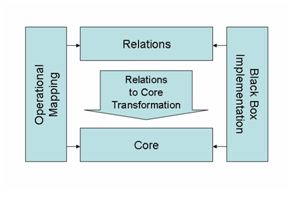
\includegraphics[scale=0.55]{content/images/Chapter3/figure1}}
\caption{Overview of different languages in QVT \cite{eclipseqvt}}
\label{fig:overview}
\end{figure}

\subsection{Xpand}
Xpand is a language released as an Eclipse plug-in for generation of code from \gls{emf} models \cite{xpand}. In \gls{mdse}, once the models are developed, it is difficult to directly execute them. For further processing, it is required that these models should be converted into executable artifacts. The Xpand language is used for such a transformation. Though there are many template languages available, Xpand is focused on effective template development for code generation with the help of a domain-specific \gls{m2t} transformation language and good tool support. Here the templates are written and are used by the generator which runs the development workflow. In addition, the Xpand language has an inbuilt small but sufficient vocabulary. Xpand’s domain-specific features and its familiarity in high level \gls{mdsd} makes it an automatic choice over other languages. 

\subsection{PIPE2}
\gls{pipe2} is an open source, platform independent tool developed for the creation and analysis of Petri Nets \cite{bonet2007pipe}. \gls{pipe2} was developed as a research project at the Imperial College in 2003.  It is completely written in Java to make it platform independent. It also provides a simple user interface which creates, saves and loads Petri Nets in conformance with \gls{pnml} interchange format. The major advantage of \gls{pipe2} is its user friendly GUI, its platform independence and its easy extensibility feature. \gls{pipe2} also features a complete set of analysis modules to check behavioral properties, derive performance statistics and other capabilities like Petri Nets comparison and classification. It also offers modules to perform different kinds of qualitative and quantitative analysis. The research group continuously works on additional enhancements to make the tool much more effective for the Petri Nets creation and analysis.
